\documentclass[10pt,a4paper]{article}
\usepackage[utf8]{inputenc}
\usepackage{amsmath}
\usepackage{amsfonts}
\usepackage{amssymb}
\usepackage{graphicx, listings}
\usepackage{url,verbatim}
\usepackage{hyperref}
\usepackage{boxedminipage}

\begin{document}

\makeatletter

\renewcommand*{\@fnsymbol}[1]{\ensuremath{\ifcase#1\or \star\or a\or b\or
   \mathsection\or \mathparagraph\or \|\or \star\star\or \dagger\dagger
   \or \ddagger\ddagger \else\@ctrerr\fi}}

\makeatother

\title{FLAViz:\\Flexible Large-scale Agent Visualization library\thanks{We gratefully acknowledge funding provided by the DFG Project Conquaire.}\\\sc Draft version, for internal use only}

\author{Sander van der Hoog\thanks{Email: \{svdhoog\}@uni-bielefeld.de, Chair for Economic Theory and Computational Economics (ETACE), Dept. of Business Administration and Economics, Bielefeld University, Germany.}}

%\author{Krishna Raj Devkota\thanks{Email: \{kdevkota,svdhoog\}@uni-bielefeld.de, Chair for Economic Theory and Computational Economics (ETACE), Dept. of Business Administration and Economics, Bielefeld University, Germany.} \and Sander van der Hoog\footnotemark[2]}

\maketitle


\clearpage
\tableofcontents

\clearpage
\section{Introduction}
This technical report describes the release of FLAViz 0.1.0 (beta version), a new visualization library developed at the ETACE group at Bielefeld University (Economic Theory and Computational Economics). 

\subsection{Overview}
\label{Section:1}

The Flexible Large-scale Agent Visualization Library (FLAViz) is a software library developed specifically for data analysis and data visualization tasks on data that is produced by multi-agent, or agent-based, simulations (ABMs). Agent-based simulation models typically generate data across multiple dimensions, e.g. parameter sets, Monte Carlo replication runs, different agent types, multiple agent instances per type, many variables per agent, and time periods (iterations). This implies the data is structured as time series panel data sets.

We specifically designed FLAViz having in mind the data generated by agent-based simulations developed in the FLAME framework, but in principle the output data from any ABM can be used, as long as the data adheres to our file specifications.

FLAViz builds on Python pandas to deal with such high-dimensional time series panel data sets.
The data is stored as structured data using multiple hierarchical levels in the HDF5 file format.
This allows for proper data aggregation, filtering, selection, slicing, transformation, and visualization.
Various plots can be specified, e.g., time series, box plots, scatter plots, histograms, and delay plots. 

\paragraph{Headlines:}

\begin{itemize}
\item FLAViz is part of the FLAME ecology, a set of tools to develop, simulate and analyse large-scale agent-based models.\footnote{FLAME stands for Flexible Large-scale Agent Modelling Environment. The FLAME website is at: \href{www.flame.ac.uk}{www.flame.ac.uk}, FLAME software can be downloaded from the GitHub repository at: \href{http://github/FLAME-HPC}{http://github/FLAME-HPC}.}

\item FLAViz provides wrapper functionality around Python pandas to facilitate the data analysis and data visualization tasks that are typical for the time series data produced by agent-based model.
\end{itemize}


\paragraph{FLAViz provides the following features:}

\begin{itemize}
\item Easy-to-configure \url{yaml} files

\item Fully written in Python (support for both Python 2.7 and 3.6)

\item Based on Python pandas (0.21.0) and matplotlib as standards for data analysis and visualization

\item Data conversion from XML files to HDF5 files

\item Data transformations of agent variables

\item Data selection based on data values or indices (e.g., select all data at iteration $t=x$, or select all data for agent $ID=i$)

\item Data filtering based on conditions (e.g., filter the selected data on the condition that agent variable X<value)

\item Data visualization using various plotting styles: time series, box plots, scatter plots, table output
\end{itemize}


\paragraph{Version history:}
\begin{verbatim}
March 1, 2018: FLAViz 0.1.0 (beta version)
\end{verbatim}


\paragraph{Disclaimer:} The functionality of this software has only been tested under Unix/Unix-like systems. It has not been tested for Windows and therefore there is no guarantee of proper execution for such systems.

\paragraph{Dependencies:}

\begin{verbatim}
Python (3.6)
Python pandas (0.21.0)
matplotlib
hdf5
PyTables
\end{verbatim}

\paragraph{File listing:}

\smallskip
Main files:
\begin{verbatim}
main.py
summarystats.py
plots.py
transform.py
\end{verbatim}

Configuration files (user-created):
\begin{verbatim}
config.yaml
plot.yaml
transform.yaml
\end{verbatim}

Other utility scripts (data transformations):
\begin{verbatim}
gendb.py               - convert XML to SQLite db
db_hdf5_v1.py          - convert db to h5 (per run)
db_hdf5_v2.py          - convert db to h5 (per agent type)
genxml.py              - convert db to XML
merge_hdf_agentwise.py - convert h5 (per run) to h5 (per agent type)
xml_hdf5.py            - convert XML to h5 (per run)
\end{verbatim}


\subsection{Data Workflow \& Data Modules}

\begin{itemize}
\item Fig. \ref{Fig: Simulation workflow} shows the simulation workflow, reflecting the order in which data is being generated, processes and visualized. This all relates to data in storage).

\item Fig. \ref{Fig: Data processing} shows the data process flow, i.e. the order in which FLAViz uses the data. We adopt the ETL process. Even though the data extraction takes time, and it is common to execute the three phases in parallel, we have not yet done so. Our ETL is therefore still a sequential process.

\item Fig. \ref{Fig: Package diagram} shows the FLAViz package diagram, showing the interconnections between the various modules.
\end{itemize}

The software package consists of several modules, related to the different tasks, as shown in blue font in Fig. \ref{Fig: Package diagram}:

\begin{itemize}
\item The \textbf{Main Module} performs that main tasks of data read-in from file, filtering the data by agent, variables, filtering conditions, and data selections.

\item The \textbf{Summary Module} computes summary statistics.

\item The \textbf{Transformation Module} performs data transformations.

\item The \textbf{Plot Module} performs all tasks related to data visualization and table output.
\end{itemize}


\begin{figure}
\graphicspath{{./png/}}
%
\begin{boxedminipage}{14cm}
\centering\leavevmode
%\vspace{.5cm}
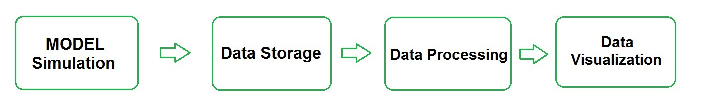
\includegraphics[scale=1]{simulation_workflow.pdf} 
\end{boxedminipage}
\label{Fig: Simulation workflow}
\caption{\footnotesize Simulation flow.}
\end{figure}

\begin{figure}
\centering\leavevmode
\graphicspath{{./png/}}
%
\begin{boxedminipage}{14cm}
\centering\leavevmode
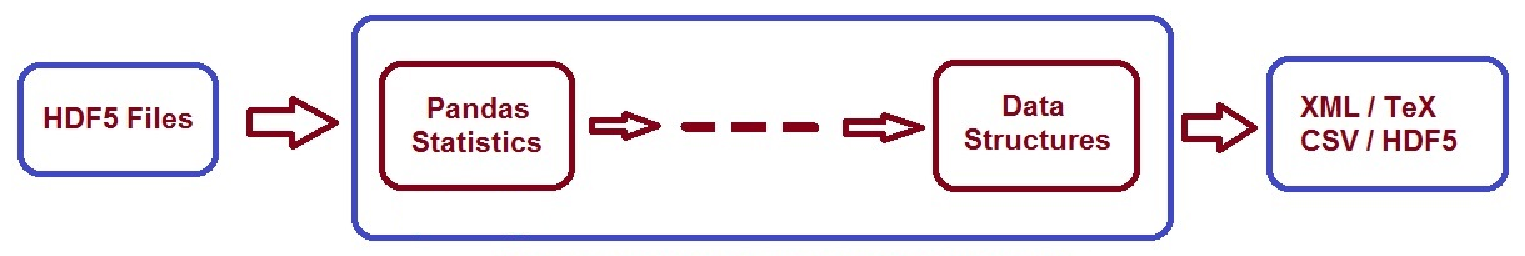
\includegraphics[scale=.5]{data_processing.pdf} 
\end{boxedminipage}
\label{Fig: Data processing}
\caption{\footnotesize Data processing flow. We follow the Extract-Transform-Load (ETL) process from data warehousing. Data extraction is where data is extracted from storage (left-most part, HDF5 files). Data transformation takes place in memory (middle part, using data frames and Python pandas). Data loading is where the trasnformed data is again written to storage (right-most part, different file formats).}
\end{figure}


\begin{figure}[Htp!]
\centering\leavevmode
\graphicspath{{./png/}}
%
\begin{boxedminipage}{16cm}
\centering\leavevmode
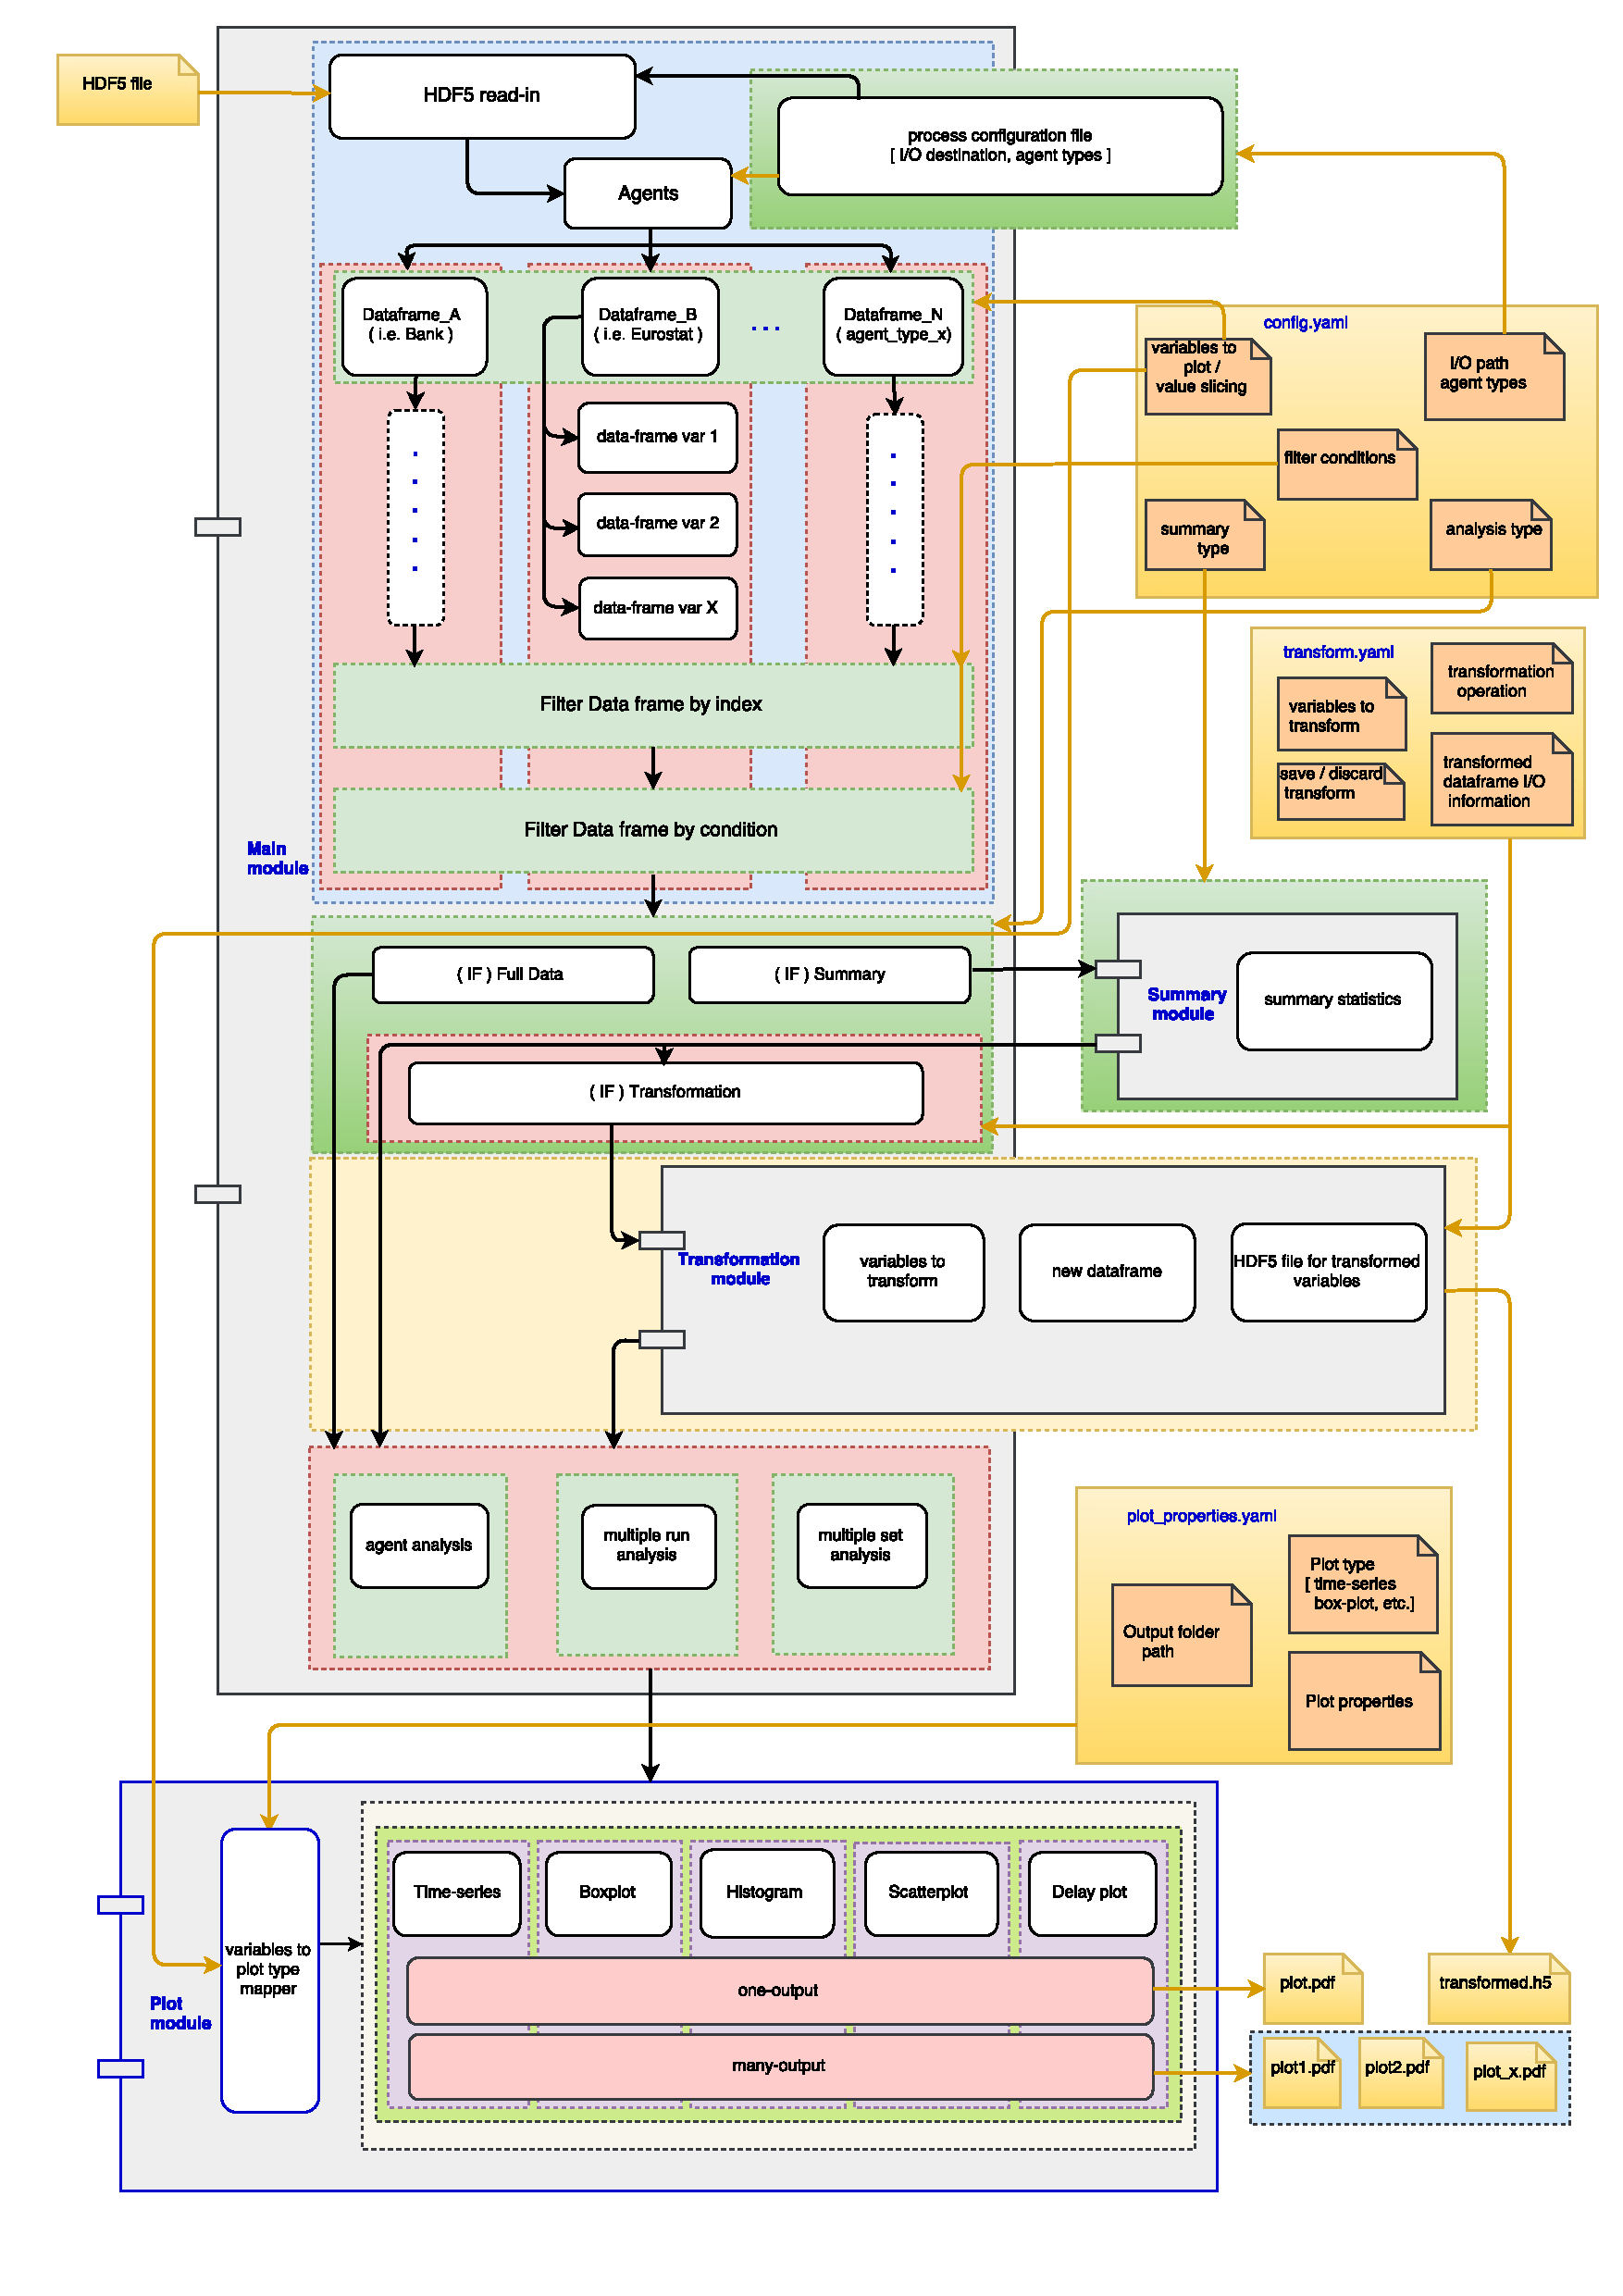
\includegraphics[scale=.4]{flavis_package_diagram.pdf} 
\end{boxedminipage}
\label{Fig: Package diagram}
\caption{\footnotesize FLAViz package diagram.}
\end{figure}



\subsection{File structure}

This package consists of several Python scripts, located in the folder \url{/src}, dealing with different steps of the data visualisation and data transformation process:
\begin{itemize}
\item \url{main.py} : Contains code to read in the input data and primary configuration files (\url{config.yaml,transform.yaml}), filter the data based on filter conditions, and link the different Summary, Plot, and Transformation modules (see Fig. \ref{Fig: Package diagram}).

\item \url{summarystats.py} : Takes in a Pandas dataframe, and computes the summary, and outputs the result as a Pandas dataframe.

\item \url{plots.py}: Takes in a Pandas dataframe, and returns the necessary plots as specified in \url{config.yaml} and \url{plot.yaml}.

\item \url{transform.py} : Takes in a Pandas dataframe, and returns/writes to a file the data transformations specified in \url{transform.yaml}.
\end{itemize}

The configuration files are contained in a folder named \url{/config}, containing three configuration files:
\begin{itemize}
\item \url{config.yaml} : defines \url{i/o} \url{path}, \url{plot-types}, \url{agents} and specifies variables, filter options, summary.

\item \url{plot.yaml} : defines plot properties i.e. \url{name, legends, line style, fill}, etc.

\item \url{transform.yaml}: defines variables to transform, type of data transformations, and \url{i/o} info to store data in a file after transformations.
\end{itemize}

Note: Further details on how to use the configuration (\url{yaml}) files can be found in Section \ref{Section:1.2} of this documentation.

\subsection{Running the main module}

To run the main executable, simply use:

\begin{lstlisting}
   $ python main.py path_to_configure_files
\end{lstlisting}

where, \url{path_to_configure_files} is the path to the folder containing the \url{yaml} configuration files.

\section{Data formats: Inputs and Outputs}
\label{Sec: Data formats}

\subsection{FLAME output data}
Fig. \ref{Fig: Simulation workflow} shows the simulation workflow. The data is generated by a simulation model, and then stored to disk. The native data output format of FLAME simulations is XML, and the default data consists of all values of all memory variables for all agents. This is called a snapshot of the agent population. A simulation run consists of many iterations, and therefore FLAME produces many XML files, each file being a snapshot at the end of an iteration. The default setting of outputting a snapshot for every iteration can be ameliorated somewhat by selecting a subset of agent types, or a subset of memory variables to be outputted. Also a certain output frequency can be selected, which may help to further reduce the data deluge.

After data storage of the per-iteration XML files, the files can be transformed into a single SQLite database file, to collect all data belonging to one simulation run.
A Python script that does the conversion from XML to SQLite is the \url{gendb.py} script.

\subsubsection{Simulation data}
We adopted the following ontology to describe how we run simulations:

\begin{itemize}
\item "Sets": a set reflects a model parameter setting. Each set differs from another set only in the parameter setting of the model.

\item "Runs": a run is a replication, for a fixed parameter setting. Each run differs from other runs by the random seed only. The other initial conditions are kept exactly the same across runs.
\end{itemize}

Thus, parameter variations are captured in "settings" or "sets". Each set reflects a different parametrization of the simulation model.
If we have any stochasticity in the model, we need to explore the statistical properties using the random seed for the Random Number Generator.
By default we use the RNG from the GNU/GSL library (a Mersenne Twister, mt19937, with a periodicity of $2^{19937} - 1$).

For each set, we then perform multiple runs using different random seeds, producing different simulation output for each run.
These runs can be called Monte Carlo replication runs since the random seeds are themselves varied in a random fashion.
The seed is set randomly based on the system time at launch time, and then stored for later replication of the data if needed.


\subsubsection{Data heterogeneity}
The data is heterogeneous across several dimensions:

\begin{itemize}
\item agent types: there can be many different agent types (e.g., household agents, firm agents, bank agents, etc.)

\item agent instances: there can be a different number of individual agents (called agent instances) per agent type.

\item agent memory variables: there can be a different number of memory variables per agent type (but all agents of the same type have the same set of memory variables, specified a priori in the model.xml file that fully specifies the model's structure).
\end{itemize}

Due to this large data heterogeneity the file sizes may vary across simulations with the same model, even when using exactly the same input file, due to stochasticity.


\subsubsection{Data dimensions in the XML output}
(listed in the order in which data is being produced by FLAME):

\begin{verbatim}
1 Sets
2 Runs
3 Iterations
4 Agent types
5 Agent instances per type
6 Variables
\end{verbatim}

However, due to several conditions we have to impose on the data structure, the order in which data should be stored in the HDF5 file format differs from the order above.
There are two restrictions:

\begin{itemize}
\item[1.] For the HDF5 file format it is important that the atomic data set at the lowest hierarchical level is a homgeneous data format.
This means that the choice of the 6 dimensions above requires us to choose those dimensions that remain invariant across all model simulations.
These dimensions are: 5 Agent instances, 3 Iterations, 6 Variables. These dimensions are invariant because we simulate the same model many times, and we do not change the model structure across simulations.
Therefore the number of variables per agent remains the same, the number of agent instances (individual agents) per agent type is constant, and the total number of iterations also remains constant across simulation runs.

\item[2.] The 3D DataFrame format in Python pandas is specified as row-major. This means that the 3D data frame requires the largest dimension to be on the major axis (recall it has 3 axis; item, major and minor).
In our case, the largest dimension is the number of iterations, typically 1000 or higher. The other dimensions are the number of agent instances (~100), and the number of variables (~100).
\end{itemize}

Therefore, we specify the 3D DataFrame as follows:\footnote{As of version 0.22.0, Python pandas is deprecating the data structure of the 3D DataFrame (or DataPanel), in favour of using the ndarray data structure. The scripts of FLAViz would have to be adapted in future releases to accommodate for this change.}
\begin{itemize}
\item item axis: agent instances
\item major axis: iterations (table rows of the DataFrame)
\item minor axis: variables (table columns of the DataFrame)
\end{itemize}

\subsubsection{Data dimensions in the HDF5 file}
 (listed in the order in which data is stored in the HDF5 files)

\subsubsection*{Agent type: HDF5 filename (eg., Bank.h5)}

Hierarchy inside the HDF5 file:
\begin{verbatim}
1 Sets: data group
2 Runs: data set inside data group
\end{verbatim}

Hierarchy inside the pandas 3D DataPanel:
\begin{verbatim}
3 Agent instances
4 Iterations
5 Variables
\end{verbatim}

\subsubsection{File format specifications}

\paragraph{Step 1: XML output}

This is the native format in which FLAME generates output. Each iteration produces an XML file that contains a full snapshot of all agents, and all agent memory variables. This can be a large file per iteration, so therefore FLAME also provides the possibility to only output one XML file at a certain frequency. This can be accomplished using the command:

\begin{verbatim}
main -f freq
\end{verbatim}

where \url{main} is the simulator executable and \url{freq} is an integer number specifying the periodicity with which output should be generated.
To further sub-sample the data outputted, it is possible to select only a subset of agents to output, or even to specify a \textbf{shadow model xml file} with only a subset of agent variables. Whatever method chosen, the data format is XML with fully tagged variables for each individual agent. Since the XML tags are rather verbose and redundant (of the format: \url{'<variable_name>value</variable_name>'}). This format can be reduced drastically by extracting the data to a more structured data format.

\paragraph{Step 2: HDF5-per-run files}

In this step we store data in one HDF5-per-run file per simulation run.

Each simulation run in FLAME produces a set of XML files, one file per iteration. This set can be tansformed into a flat table format, with iteration number on the table rows, and all variables of an individual agent on the table columns.
This would produce many tables, as many as there are individual agents. To reduce this further, we structure the data using the following dimensions (see also above, Data dimensions in the HDF5 file):

File hierarchy:
\begin{verbatim}
1 Set
2 Run
4 Agent type
\end{verbatim}

Inside each HDF5-per-run file:
\begin{verbatim}
5 Agent instance
3 Iteration
6 Variable
\end{verbatim}


\paragraph{Step 3: HDF5-per-agent-type files}

In this step we store data in one HDF5-per-agent-type file. this aggregates across all the files generated at the previous step 2 (all HDF5-per-run files).

Structure:
\begin{verbatim}
HDF5 file:
Data group: "Sets" (parameter setting)
Data set:   "Runs" (replications) stored as 3D DataPanel
\end{verbatim}


\begin{verbatim}
3D DataPanel:
item axis: agent instances
major axis (table rows): iterations
minor axis (table columns): variables
\end{verbatim}



\subsection{Data preparation}

The FLAViz library can only deal with input data that is stored in \emph{HDF5} container files (\url{.h5} or \url{.hdf5} file extension). The data inside such a file is stored using a hierarchical format. Currently, the HDF5 file has to be structured as follows:
\begin{itemize}
\item Data for each agent-type is stored in a separate HDF5 file, with the same name as the agent type name.

\item Each HDF5 file has a single hierarchy, with the \emph{agent-type} as the root, and the \emph{set} and \emph{runs} as the sublevels. Inside the HDF5 hierarchy, the sets are stored as a 'data set', and the runs are stored as a data group.

\item At the lowest level of the HDF5 hierarchy is a variable of type \emph{DataPanel}, which is Python pandas 3D data structure. This DataPanel itself contains three dimensions, also called \url{axes}: \url{major, minor}, and \url{items}.

\item The 3D DataPanel data structure is written to the HDF5 file with the help of the \emph{PyTables} module in Python.\footnote{For performance reasons we use PyTables in 'fixed' write-only mode that does not allow to append data to the HDF5 file lateron. An alternative would be to use the 'append' mode, but our tests have shown that this incurs a considerable degradation in the I/O performance.}
\end{itemize}

\paragraph{Note:} An HDF5 file as specified above can be created from raw data to the \url{h5} format, either by using the script \url{db_hdf5_v1.py} to convert SQLite \url{db} files, or by using the script \url{xml_hdf5.py} to convert the XML files directly. Both Python scripts are included in the data processing directory.

\subsubsection{Data conversion scripts}

The folder \url{data_conversion_scripts/} contains a set of Python scripts to translate between various file formats.
The conversion scripts currently included are:
\begin{verbatim}
gendb.py               - convert XML to SQLite db
db_hdf5_v1.py          - convert SQLite db to h5 (per run)
db_hdf5_v2.py          - convert SQLite db to h5 (per agent type)
genxml.py              - convert SQLite db to XML
merge_hdf_agentwise.py - convert h5 (per run) to h5 (per agent type)
xml_hdf5.py            - convert XML to h5 (per run)
\end{verbatim}


\subsubsection*{Dependencies}
The scripts have been tested to work with both Python \url{2.7.10} / Python \url{3.5.2} and above.

The required dependencies are:
\begin{verbatim}
Pandas >= 0.19.2
scipy >=0.18.1
numpy >= 1.11.3
\end{verbatim}

The data storage format requires the following dependency:

\begin{verbatim}
pytables
\end{verbatim}

\subsection{Usage of the conversion scripts}

\paragraph{Note:}
To avoid any unwanted errors, it is imperative to name the SQLite database files using the following convention:

\begin{verbatim}
set_s_run_r_iters.db
\end{verbatim}
where $s$ is the set number and $r$ is the run number.
 
\subsubsection{Converting files: per-run SQLite db to per-run h5}
The script \url{db_hdf5_v1.py} converts a folder with \textbf{per-run} \url{db} files, creating a single HDF5 file in many-to-one fashion.
So for all the data content in the db files present in one folder, the data is combined into one equivalent HDF5 file in the output folder. 
If the input folder contains a folder hierarchy, and if the recursive mode flag \url{-r} is set, then one HDF5 file is created for the contents of each subfolder.

\begin{itemize}
\item Input files: \url{input_folder/set_*_run_*_iters.db}

\item Output files: \url{output_folder/iters.h5}
\end{itemize}

Example usage:
\begin{verbatim}
# Converts the SQLite database files to HDF5 files.
# Combines multiple db files into a single HDF5 file.
# Usage: db_hdf5_v1.py [-h] [-o OUTPATH] [-v] [-s] dbpath
# dbpath             : Path to folder containing the .db files
# outpath            : Path to folder for the output .h5 files
# '-o', '--outpath'  : Path to the folder where the output is desired
# '-v', '--verbose'  : Get the status of the intermediate processing steps
# '-s', '--status'   : Get the total progress of the processing
# '-r', '--recursive': Recursively process all subfolders within the input folder

# Example 1: non-recursive input folder
python3 db_hdf5_v1.py -o h5/ -v -s db_iters_files/

# Example 2: recursive input folder
python3 db_hdf5_v1.py -o h5/ -v -s -r db_iters_files/
\end{verbatim}

\subsubsection{Converting files: per-run SQLite db to per-run h5}
The script \url{db_hdf5_v2.py} converts \textbf{per-run} \url{db} files into the corresponding \textbf{per-run} \url{h5} format. By default, the script traverses a folder from its root into the entire folder hierarchy, searching for any \url{*.db} files in its subfolders, and converting these into their corresponding \url{*.h5} files.
\begin{itemize}
\item Input files: \url{set_*_run_*_iters.db}

\item Output files: \url{set_*_run_*_iters.h5}
\end{itemize}

Example usage:
\begin{verbatim}
# Convert iters.db to iters.h5
# Usage: db_hdf5_v2.py [-h] [-o OUTPATH] [-v] [-s] dbpath
# -v: verbose mode, provides info on agent processed and overall progress
#     in folder if multiple files present
# -s: status, provides info on file output status

# Example:
python3 db_hdf5_v2.py -o h5_iters_files/ -v -s db_iters_files/
\end{verbatim}

\subsubsection{Converting files: h5 per-run to h5 per-agent-type}
The script \url{merge_hdf_agentwise.py} converts \textbf{per-run} h5 files to \textbf{per-agent-type} h5 files.
\begin{itemize}
\item Input files: 
	\begin{itemize}
	\item \url{set_*_run_*_iters.h5}: per-run h5 files.
	\item \url{agent_list.txt}: a plain text file with a list of agent types to be converted (one per line).
	\end{itemize}
\item Output files: \url{Agentname.h5}: per-agent type h5 files.
\end{itemize}

Example usage:
\begin{verbatim}
# Usage: merge_hdf_agentwise.py [-h] [-o OUTPATH] [-v] [-s] dbpath
# hdfpath: Path to folder containing the individual hdf files
# agentlist: File containing name of agent-types to process
# -o, --outpath: Path to the folder where the output is desired
# -v, --verbose: Get the status of the intermediate processing steps
# -s, --status: Get the total progress of the processing

# Example:
python3 merge_hdf_agentwise.py -o h5_agentwise -s h5_iters_files/ agent_list.txt
\end{verbatim}


\subsubsection{Results}

\begin{itemize}
\item Fig. \ref{Fig: h5 per run list} shows the output of the script \url{db_hdf5_v2.py}, which produces a list of per-run \url{h5} files.

\item Fig. \ref{Fig: h5 per run contents} shows the contents of a per-run \url{h5} file. For the selected agent type \url{Bank}, the panel on the right-hand side shows the contents of the 3D DataPanel with the \url{major} axis (iterations), the \url{minor} axis (agent instances, 20 in this case), and the \url{item} axis (data content). Note that the data content is not clearly descernible because we have used the internal data compression for the HDF5 format. This clearly reduces the storage requirement, but makes the resulting \url{h5} files non-viewable.

\item Fig. \ref{Fig: h5 per agent list} shows the output of the script \url{merge_hdf_agentwise.py}, which produces a list of per-agent-type \url{h5} files.

\item Fig. \ref{Fig: h5 per agent contents} shows the contents of a per-agent-type \url{h5} file. The selected HDF5 data set corresponds to the agent type \url{Eurostat}, and the selected HDF5 data group is \url{set_1_run_1_iters}. The panel on the right-hand side shows the contents of the 3D DataPanel. The data in the \url{item} axis (third axis) is now decipherable, because in this case no internal data compression was used when writing to the HDF5 data format.
\end{itemize}


\begin{figure}[htb!]
\centering\leavevmode
\graphicspath{{./hdf5_snapshots/}}
%
%\begin{boxedminipage}{16cm}
\centering\leavevmode
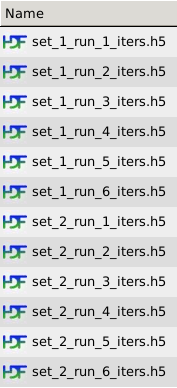
\includegraphics[scale=.4]{Fig_0_list_of_separate_hdf5_files.png} 
%\end{boxedminipage}
\label{Fig: h5 per run list}
\caption{\footnotesize Output of the script \url{db_hdf5_v2.py}: List of h5 files per run.}
\end{figure}


\begin{figure}[htb!]
\centering\leavevmode
\graphicspath{{./hdf5_snapshots/}}
%
%\begin{boxedminipage}{16cm}
\centering\leavevmode
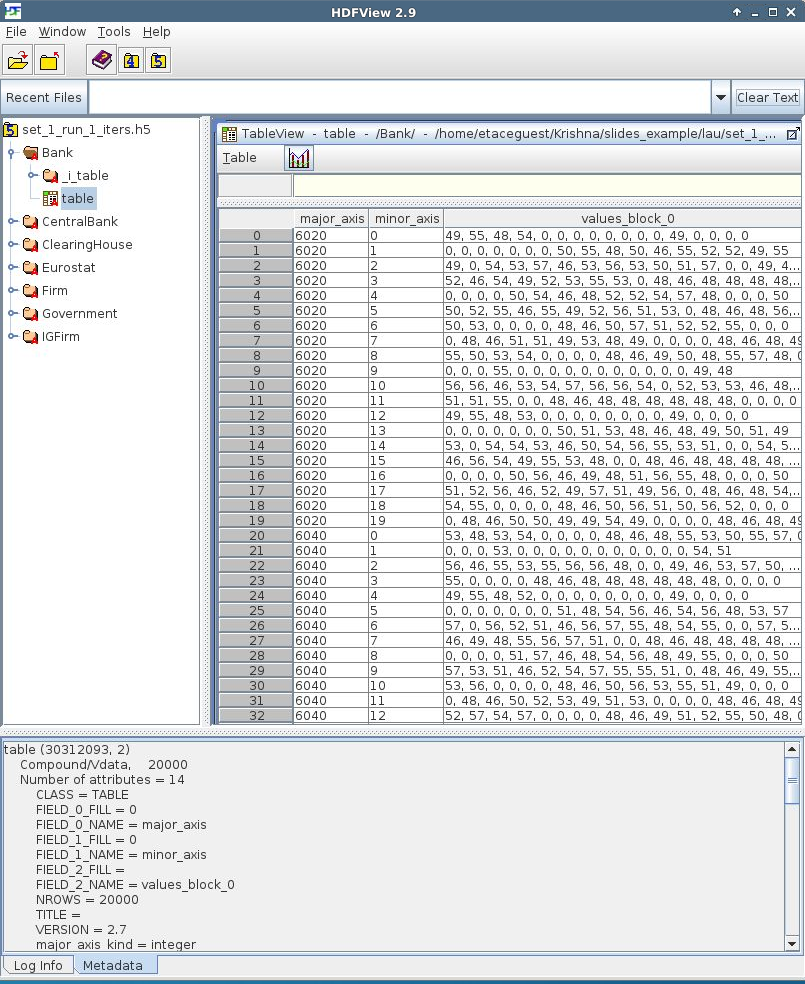
\includegraphics[scale=.4]{Fig_1_individual_hdf5_corresponding_to_db_agent_1.png} 
%\end{boxedminipage}
\label{Fig: h5 per run contents}
\caption{\footnotesize Output of the script \url{db_hdf5_v2.py}. The 3D DataPanel on the right shows the contents of the HDF5 data set \url{set_1_run_1_iters}, for the data group \url{Bank}. The data in the third axis of the 3D DataPanel, i.e. the \url{item} axis, is non-decipherable because we used the internal data compression of the HDF5 data format when writing the output to the file.}
\end{figure}


\begin{figure}[htb!]
\centering\leavevmode
\graphicspath{{./hdf5_snapshots/}}
%
%\begin{boxedminipage}{16cm}
\centering\leavevmode
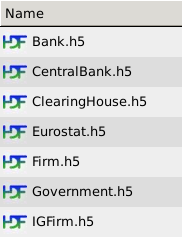
\includegraphics[scale=.4]{Fig_4_list_of_hdf5_files_separated-per-agent-type.png} 
%\end{boxedminipage}
\label{Fig: h5 per agent list}
\caption{\footnotesize  Output of the script \url{merge_hdf_agentwise.py}: List of h5 files per agent type.}
\end{figure}


\begin{figure}[htb!]
\centering\leavevmode
\graphicspath{{./hdf5_snapshots/}}
%
%\begin{boxedminipage}{16cm}
\centering\leavevmode
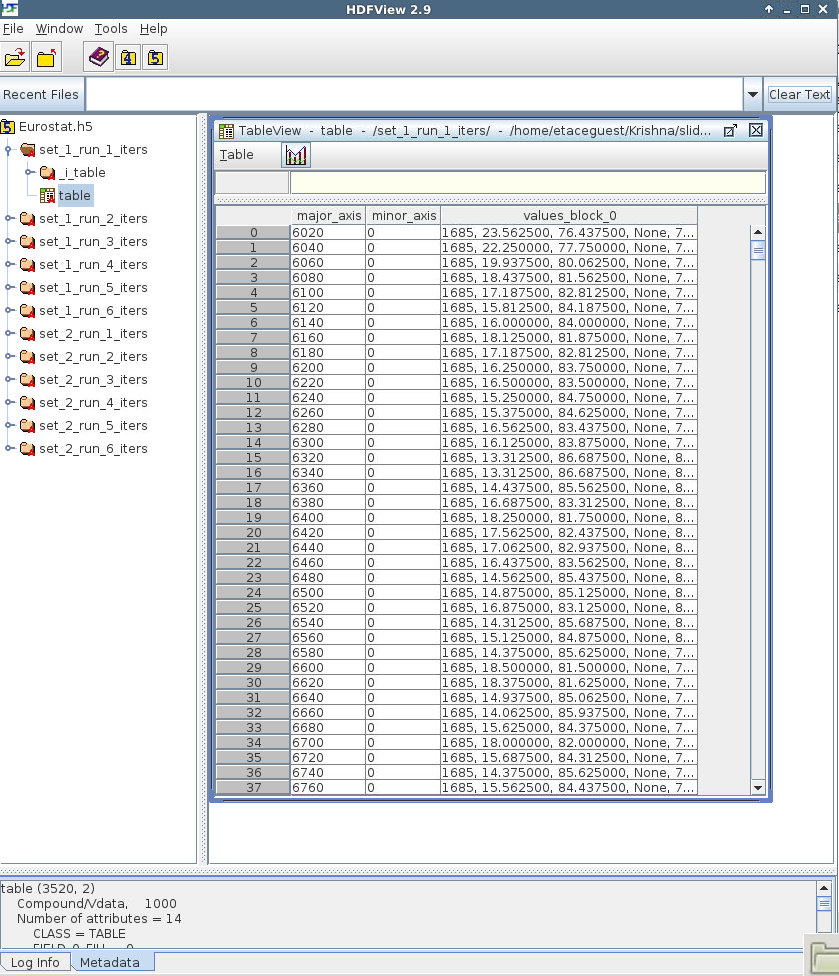
\includegraphics[scale=.4]{Fig_3_hdf5_file_per_agent_showing_values.png} 
%\end{boxedminipage}
\label{Fig: h5 per agent contents}
\caption{\footnotesize Output of the script \url{merge_hdf_agentwise.py}; contents of the HDF5 file for agent type Eurostat. The 3D DataPanel on the right shows the contents of the HDF5 data set \url{Eurostat}, for the data group  \url{set_1_run_1_iters}. The data in the \url{item} axis (third axis) is decipherable, because in this case no internal data compression was used when writing to the HDF5 data format.}
\end{figure}


\subsection{Performance benchmarks}

In this section we report on the performance of the process of transforming the SQLite database files (\url{*.db}) to HDF5 files (\url{*.h5}).
This process consists of three sub-processes. 

In the first sub-process (data preparation), the data structures required for the further processing of data lateron is being prepared. This involves parsing the model XML to read the agent types, their memory variables, and to allocate memory for the dataframe that will be filled in with values from the SQLite database files. This process is independent of the size of the problem.

In the second sub-process (extracting and transforming the data), the SQLite database files are read-in from hard disk storage. This process is linear in the number of sets to process. Each file is extracted from storage, stored in memory, and then transformed into the native data format that is used by Python pandas, which is a flat table format, or dataframe. This dataframe can have an hierarchical index with 6 indices, as described in Section \ref{Sec: Data formats}.

In the third sub-process (loading the data), the flat, hierarchical dataframe is transformed into the format of the 3D DataPanel, and then written out to HDF5 files.

Fig. \ref{Fig: Performance} and Table \ref{Tab: Performance} show performance benchmarks for the Extract-Transform-Load process described above. We used sets of different sizes, i.e. the number of sets. Each set consisted of $1,0000$ runs of an ABM simulation, for $20,000$ iterations. Each ru takes aprox. 20 min, to complete, and yields a single output file of 64kb.\footnote{The data used for these performance benchmarks is available in the data publication van der Hoog, S. and Barde, S., 2017, Data for the paper: An empirical validation protocol for large-scale agent-based models, Bielefeld University.  \url{https://10.4119/unibi/2908396}. The data for the 513 sets is contained in these files:
\url{calibration-mode-3-stage-1-sets-1-256-tarballs-part-1.tar.bz2} (7.47 GB) and \url{calibration-mode-3-stage-1-sets-257-513-tarballs-part-2.tar.bz2} (7.5 GB).}

We considered only 3 cases, with 100, 250 and 513 sets, resp. For the largest case with 513 sets, the first 90 min./5 GB are used to read in the files from storage. After that, the transformation from flat 2D dataframes to the 3D DataPanel format takes about 260 min./145 GB. The final process of writing out the results to HDF5 takes approx. 50 min./50 GB.

\begin{table}
\label{Tab: Performance}
\begin{tabular}{|c||cc||cc||cc|}
\hline \hline 
Process:  & \multicolumn{2}{|c|}{Preparation} & \multicolumn{2}{|c|}{Extract \& Transform} & \multicolumn{2}{|c|}{Load}\\ 
\hline 
No. sets  & Time (min.) & RAM (GB) & Time (min.) & RAM (GB) & Time (min.) & RAM (GB)\\ 
\hline 
100 & 90 & 5 & 50 & 25 & 10 & 10\\ 
\hline 
250 & 100 & 5 & 130 & 70 & 25 & 25\\ 
\hline 
513 & 90 & 5 & 260 & 145 & 50 & 50\\ 
\hline 
\end{tabular} 
\caption{Performance benchmarks for the data extraction from storage and the data processing in RAM memory.}
\end{table}



\begin{figure}[htb!]
\centering\leavevmode
\graphicspath{{./Benchmarks/}}
%
%\begin{boxedminipage}{16cm}
\centering\leavevmode
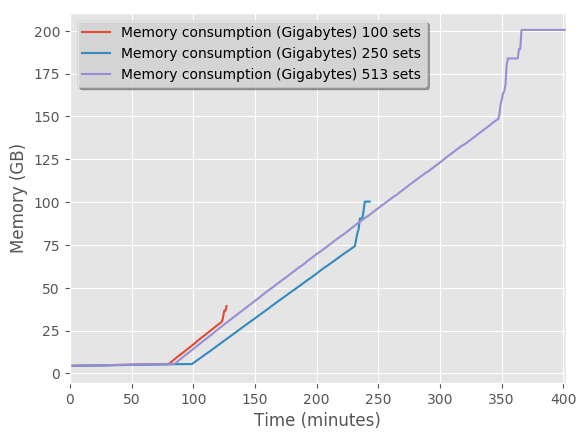
\includegraphics[scale=.9]{Fig_all.png} 
%\end{boxedminipage}
\label{Fig: Performance}
\caption{\footnotesize Performance benchmark for the ETL process.}
\end{figure}

\clearpage
\section{FLAViz Configuration files}
\label{Section:2}
There are three configuration files, which allow the user to input the necessary parameters for the program. The configuration files are specified in the \url{yaml} format that uses a hierarchical format which is not just for clarity but also for specifying functionality. Hence, it is important to abide by the indentation of the yaml files in order for them to be interpreted correctly. 

\paragraph{Note:} Any error in a \url{yaml} file might be caught by the exception handler, but indentation errors go unnoticed sometimes, which may result in undesired output. Hence, extra care is advised when formulating a configuration file.

\subsection{File: config.yaml}

\subsubsection*{Data input/output section}

\url{i/o}: Specify the input and output path.

\begin{itemize}
    \item The input path is specified as a full path in the sub-hierarchy \url{input_path}:
\end{itemize}

\lstset{language=C,frame=single, basicstyle=\footnotesize}
\begin{lstlisting}
  i/o:
    input_path:   '/home/etace'

    input_files: 
        Bank:     'Bank.h5' 
        Eurostat: 'Eurostat.h5'
\end{lstlisting}
\paragraph{Note:} The key name to the input path should correspond to the Agent-type (e.g., Bank, Eurostat, Firm etc.)

\begin{itemize}
    \item The output path is specified as a full path in the sub-hierarchy \url{output_path}:
\end{itemize}

\begin{lstlisting}
    output_path: '/home/etace/timeseries'
\end{lstlisting}    


\subsubsection*{Plot section}

\begin{lstlisting}
    plot1:
        timeseries:
            agent: Bank
            analysis: multiple_set
            variables: 
              var1: [total_credit]  
              var2: [equity]
\end{lstlisting}    
 
\begin{itemize}
    \item \textbf{Plot-key} (e.g., \url{plot1}): Specify a key for the plot (mainly to keep track of the plot-number for other configuration files). Can be any string.
    \item \textbf{Plot-type} (e.g., \url{timeseries}): Nested under \textbf{Plot-key} (here \url{plot1}), "Plot-type" specifies the type of plot desired.
	\begin{itemize}
		\item Possible values: \url{timeseries, boxplot, histogram, scatterplot}.
	\end{itemize}
\end{itemize}

\paragraph{Note [Exception]:} For data transformations, simply specify \url{transform} as the Plot-type, and it will perform the transform and store the new data items to a specified output file (no plots will be produced). 
\begin{lstlisting}
    plot1:
        transform:
            agent: Bank
            analysis: multiple_set
            variables: 
              var1: [total_credit]  
              var2: [equity]
\end{lstlisting}    

\begin{itemize}
    \item \url{agent}: Name of the agent-type, nested under \textbf{Plot-type}.

    \item \url{analysis}: Type of analysis. Possible types:  \url{agent, multiple_run, multiple_batch, multiple_set}.

    \item \url{variables}: Variables from the particular agent-type to be processed or visualized. The sub-hierarchy \url{var1, var2} etc. allows the input of multiple variables for any agent type.
    The variable names can be inside a set of square brackets \url{[]} or simply inside a set of single-quotation marks \url{''}.
\end{itemize}


\subsubsection*{Conditional filtering}
The option to filter variables is based on filter conditions on the values, i.e. to retrieve only those values satisfying certain restrictions or are within a certain range. For conditional filtering, specify the variables as above, but with the filter conditions in addition.

\begin{itemize}
    \item Possible operator types are: \url{<,>,<=,>=,==}.
    \item Simple or multiple filter conditions on a variable are possible.
    \item Filtering on multiple variables can be specified.
\end{itemize}
        
\begin{lstlisting}[caption={Filtering examples using single and multiple filter conditions.}]
    var1: [variable name, 'operator[value]']
    e.g.
    var1: [total_credit, '>[700]'] 
    # Select only values of total credit greater than 700.
    
    var2: [variable name, 'operator1[value]','operator2[value]']
    e.g.
    var2: [equity, '>[700]', '<[1500]'] 
    # Select only values of total credit between 700 and 1500.
\end{lstlisting}    

\begin{lstlisting}[caption={Filtering example using multiple variables.}]
    plot1:
        timeseries:
            agent: Bank
            analysis: multiple_set
            variables: 
                  var1: [total_credit, '>[700]']  
                  var2: [equity, '>[700]', '<[800]']
\end{lstlisting}    

\subsubsection*{Data selection}
For the \textbf{sets}, \textbf{runs}, \textbf{major} and \textbf{minor} axes, the data selection can be specified either as a ranges or as a list:\footnote{The third axis of the 3D DataPanel, the \url{item} axis, is deliberately left out of this list for data selections, since it is used to store the variables. These can be selected separately under the \url{'variables'} section in the \url{config.yaml} file.}
\begin{itemize}
\item \url{set} : Specify the sets to process. Input can be an explicit list, or (esp. for long lists) a custom way is to specify a range of values.

\item \url{run} : Specify the runs to process. Syntax is similar to \url{sets} above.

\item \url{major} : Specify the values from the major axis (iterations). Syntax similar to \url{sets} above.

\item \url{minor} : Specify the values from the minor axis (agent instances). Syntax similar to \url{sets} above.
\end{itemize}

Example of selecting sets using an explicit list of values:
\begin{lstlisting}
    set: [val(1),val(2),...,val(N)]
    e.g.
    set: [1,2]
\end{lstlisting}    
    
Example of selecting sets using a range of values (list with values from 1 to 10 with a step size of 2):
\begin{lstlisting}
    set: [range,[val(1),val(N),stepsize]]
    e.g.
    set: [range, [1,10,2]]
\end{lstlisting}  
\paragraph{Note:} The \url{set,run,major}, and \url{minor} values are nested under "Plot-type"

\bigskip
\textbf{Full example for data selection:}
\begin{lstlisting}
    plot1:
        timeseries:
            agent: Bank
            analysis: multiple_set
            variables: 
                  var1: [total_credit]  
                  var2: [equity]     
            set: [1]
            run: [1,2]
            major: [range,[6020,26000,20]]
            minor: [1,5,7] # only consider agents 1,5,7
\end{lstlisting}

\begin{itemize}
\item \url{summary}: Specify the type of statistical summary. This is also nested under Plot-type.
	\begin{itemize}
		\item Possible values: \url{mean,median,custom_quantile,upper_quartile,lower_quartile,maximum,minimum}.
	\end{itemize}
\item \url{[quantile_values]}: Specify an interquantile range
	\begin{itemize}
		\item \url{lower_quantile}: \url{[0-100]}
		\item \url{upper_quantile}: \url{[0-100]}
	\end{itemize}
\end{itemize}


\textbf{Example for summary}
To show a simple mean of the data, use:
\begin{lstlisting}
    plot1:
        timeseries:
            summary: mean
\end{lstlisting}

To show an an interquantile range, use:
\begin{lstlisting}
    plot1:
        timeseries:
            summary: custom_quntile
            quantile_values:
            	lower_quantile: 0.20
            	upper_quantile: 0.80
\end{lstlisting}


\bigskip
\textbf{Complete example config.yaml file}

A complete example \url{config.yaml} file may look like this:
\begin{lstlisting}
    i/o:
        input_path: '/home/etace/'
        
        input_files:         
            Bank:     'Bank.h5'
            Eurostat: 'Eurostat.h5'
        output_path: '/home/etace/timeseries'
        
    plot1:
        timeseries:
            agent: Bank
            analysis: multiple_set
            variables: 
                var1: [total_credit]  
                var2: [equity]     
            set: [1]
            run: [1,2]
            major: [range,[6020,26000,20]]
            minor: [1,5,7] 
            summary: mean
            
    plot2:
        boxplot:
            agent: Eurostat
            analysis: multiple_run
            variables: 
                var1: [total_credit]       
            set: [1]
            run: [1]
            major: [range,[6020,6900,20]]
            minor: [1,8] 
            summary: custom_quantile
            quantile_values:
            	lower_quantile: 0.25
            	upper_quantile: 0.75            
\end{lstlisting} 


\subsection{File: plot.yaml}

For every plot that is specified in the main configuration file \url{config.yaml}, the file \url{plot.yaml} provides further specifications for the plot (i.e., the line style, axes labels, legend placement, etc.). The \url{plot.yaml} file contains all the necessary configurations for each plot to be generated, and is linked by the \textbf{Plot-key} as specified in the \url{config.yaml} file. Below we explain the parameters from the \url{plot.yaml} file.\footnote{The plotting options follow the specifications in the \url{matplotlib} library, which is the default library to plot data with Python pandas.}

\begin{itemize}
\item \textbf{Plot-key} (e.g., \url{plot1}): This string should be the same as the \textbf{Plot-key} in the \url{config.yaml} file, to make sure the correct parameters are mapped to the respective plotting modules.

\item \url{number_plots}: Specifies how many plots will be output per variable for a particular agent type. 
\begin{itemize}
\item Possible values: \url{one,many}.
\item \url{one}: all data series will be displayed in a single plot graph. For time series plots this means: many lines in one plot graph.
\item \url{many}: each data series is displayed in a separate plot graph. There will be as many plot graphs as there are data series selected.
\end{itemize}

\item \url{plot_name}: Specify a filename for the plot.
(Note: In case of multiple plots, a numerical suffix (in increasing order) is added after the specified file name.)

\item Plotting limits:
\begin{itemize}
\item \url{l_lim}: y-axis lower limit.
\item \url{u_lim}: y-axis upper limit. 
\item \url{tmin}:  x-axis lower limit (time axis).
\item \url{tmax}: x-axis upper limit (time axis).
\item Possible values: \url{no, numeric}. (\url{no} means: automatic scaling)
\end{itemize}

\item \url{plot_legend}: Specify whether a legend for the plot should be displayed.

\item \url{legend_loc}: Specify the location of the legend, either inside or outside of the graph box.
\begin{itemize}
\item Possible values: \url{in,out}.
\end{itemize}

\item \url{legend_label}: Specify a name for the lines in the plot. Can be any string value.

\item \url{x-axis} \url{label}: Specify a label for the x-axis. Can be any combination of string values.

\item \url{y-axis} \url{label}: Specify a label for the y-axis. Can be any combination of string values.

\item \url{linestyle}: Specify line characteristics. 
\begin{itemize}
\item Possible values: \url{solid,dashed,dashdot,dotted} etc.
\end{itemize}

\end{itemize}

\bigskip
\textbf{Complete example plot.yaml file}

\begin{lstlisting}
    plot1:
        number_plots: one
        plot_name: timeseries_equity.png
        l_lim: no
        u_lim: no
        tmin: no
        tmax: no
        plot_legend: yes
        legend_loc: out
        legend_label: equity
        x-axis label: months
        y-axis label: equity value
        linestyle: solid
        
    
    plot2:
        number_plots: many
        plot_name: boxplot_monthly_output.png
        l_lim: no
        u_lim: no
        tmin: no
        tmax: no
        plot_legend: no
        legend_loc: in
        legend_label: monthly_output
        x-axis label: months
        y-axis label: monthly_output
        linestyle: dashed
\end{lstlisting}

\subsection{File: transform.yaml}

The \url{transform.yaml} file contains all the specifications for any data transformation. Whenever a transformation is specified in the \url{config.yaml} file, the \url{transform.yaml} file is read to perform the required transformations, and store the resulting data in a new output HDF5 file.

\bigskip
The parameters in the \url{transform.yaml} file are as follows:

\begin{itemize}
\item \textbf{Plot-key} (e.g., \url{plot1}): This string should be the same as the \textbf{Plot-key} used in the \url{config.yaml} file for identifying the data transformation block, to make sure the correct parameters are mapped to the respective data transformation modules.
(Note: Although it is called Plot-key, the transform case is an exception and no plots are produced in this case.)

\item \url{variables}: Variables from the particular agent-type that are to be transformed. The sub-hierarchy \url{var1,var2} etc. allows
the input of multiple variables for any agent type. 

\item \url{transform_function}: The transformation function to apply for the given variables.

\paragraph{Note:} Other elementary functions such as \textbf{sum}, \textbf{difference}, \textbf{product}, and \textbf{division} can also be performed, which has been left for the user (will be added as custom functions).

\item \url{aggregate}: If the transformation is to be performed after calculating the summary stats, then a necessary aggregation method can be specified.
\begin{itemize}
\item Possible values: \url{mean,median,maximum,minimum,custom_quantile,upper_quartile,lower_quartile}.
\end{itemize}

\item \url{write_file}: Specify whether to write the transformation to a file.
\begin{itemize}
\item Possible values: \url{yes,no}.
\end{itemize}

\item \url{output_path}: If the \url{write_file} option above is set to \url{yes}, then an output path for the file needs to be specified.
This can be any valid file path, as a string, including the filename.

\item \url{hdf_groupname}: Specify the rootname for the HDF5 group name (internal hierarchy) for the transformed variable. Can be any valid string.
\end{itemize}

\subsubsection{Definitions of data transformations}
Possible transform functions are listed in Table \ref{Table: Transformation}.

\begin{table}[hbt!]
\label{Table: Transformation}
\begin{tabular}{|c|c|l|}
\hline \hline 
Function & Formula & Description\\
\hline 
\url{q_o_q} & $\sum_{s=0}^2 x_{t-s}/\sum_{s=3}^5 x_{t-s}$ & \parbox{7cm}{Quarter-on-quarter growth rate (this quarter wrt. previous quarter, monthly data)} \\ 
\hline 
\url{q_o_q_ONE_CYCLE} & $\sum_{s=0}^2 x_{t-s}/\sum_{s=12}^{14} x_{t-s}$ & \parbox{7cm}{Quarterly growth rate (annual window, wrt. same quarter in previous year, monthly data)} \\ 
\hline 
\url{m_o_m} & $x_{t}/x_{t-1}$ &  \parbox{7cm}{Month-on-month growth rate (this month wrt. previous month, monthly data)} \\ 
\hline 
\url{m_o_m_ONE_CYCLE} & $x_{t}/x_{t-12}$ & \parbox{7cm}{Monthly growth rate (annual window,  wrt. same month in previous year, monthly data)} \\ 
\hline 
\url{annual_P_I_T} & $\sum_{s=0}^{11} x_{t-s}/\sum_{s=12}^{23} x_{t-s}$ & \parbox{7cm}{Annual growth rate} \\ 
\hline 
\end{tabular} 
\caption{Transformation functions for commonly used growth rates.}
\end{table}


\bigskip
\textbf{Complete transform.yaml file}

A particular complete \url{transform.yaml} file may look as follows:
\begin{lstlisting}
    plot2:
        variables: 
            var1: [total_credit]
            var2: [equity]       
        transform_function: m_o_m_ONE_CYCLE
        aggregate: mean    
     
        write_file: yes
        output_path: '/home/etaceguest/transformed.h5'
        hdf_groupname: 'growth_rates'
\end{lstlisting}


\clearpage
\section{Walkthrough and Tutorial examples}
\label{Section:2}

In this section we give examples of input configuration files and their respective output plots.
Once the necessary parameters are set, by following the instructions specified in Section \ref{Section:1.2}, the module can be run to get the desired results. To demonstrate some of the functionalities, the parameters of the configuration files are shown below, along with the plots they yield.

Using the dataset \url{<INSERT DATA SET URL>}, and the following parameter settings, the following plots can be produced.

\clearpage
\subsubsection{Example 1}
For agent Firm, one set, ten runs, 80 agent instances, plotted in a single plot.

\begin{lstlisting}
config.yaml::

    plot1:
        timeseries:
            agent: Firm
            analysis: multiple_run
            variables:
                var1: [price]
            set: [13]
            run: [range,[1,10]]
            major: [range,[6020,12500,20]]
            minor: [range,[1,80]] 
            summary: mean

plot.yaml::

    plot1:
        number_plots: one
        plot_name: one_set_multiple_runs_timeseries.png
        plot_legend: yes
        legend_location: best
        xaxis_label: Time
        yaxis_label: price
        linestyle: solid
        marker: None
\end{lstlisting}

\begin{figure}[b!]\centering\leavevmode
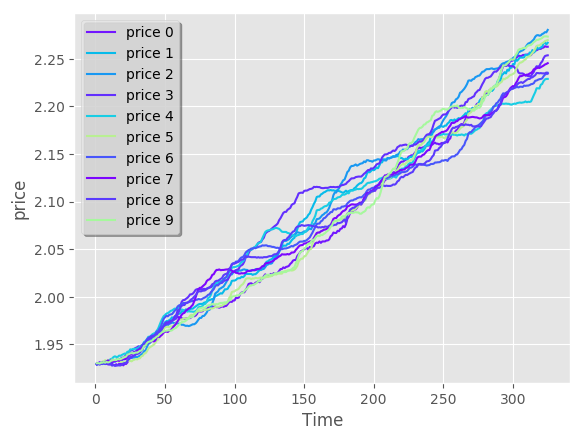
\includegraphics[scale=.7]{./plots_tut_2/one_set_multiple_runs_timeseries_price.png} 
\caption{\footnotesize  Example 1: one set, multiple runs, timeseries, price.}
\end{figure}

\clearpage
\subsubsection{Example 2}
For agent Firm, one set, one run, 20-80 quantiles of population distribution across 80 agent instances, plotted in a single plot.

\begin{lstlisting}
config.yaml::

    plot2:
        timeseries:
            agent: Firm
            analysis: multiple_run
            variables:
                var1: [price]
            set: [10]
            run: [1]
            major: [range,[6020,12500,20]]
            minor: [range,[1,80]] 
            summary: custom_quantile
            quantile_values:          
               lower_quantile : 0.20
               upper_quantile : 0.80

plot.yaml::

    plot2:
        number_plots: one
        plot_name: one_set_multiple_runs_ts_quantile.png
        plot_legend: yes
        legend_location: best
        xaxis_label: Time
        yaxis_label: price
        linestyle: solid
        marker: None
        fill_between_quartiles: yes
        fillcolor: red
\end{lstlisting}

\begin{figure}[b!]\centering\leavevmode
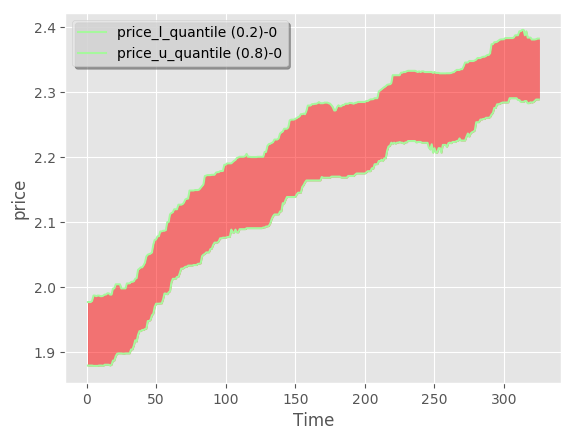
\includegraphics[scale=.6]{./plots_tut_2/one_set_multiple_runs_ts_quantile_0.png}
\caption{\footnotesize  Example 2: Quantiles 20 and 80 of the population distribution across 80 agent instances.}
\end{figure}

\clearpage
\subsubsection{Example 3}
 For agent Firm, one set, one run, 80 agent instances, boxplot.

\begin{lstlisting}
config.yaml::

    plot3:
        boxplot:
            agent: Firm
            analysis: multiple_set
            variables:
                var1: [price]
            set: [13]
            run: [1]
            major: [range,[6020,12500,20]]
            minor: [range,[1,80]]

plot.yaml::

    plot3:
        number_plots: one
        plot_name: one_set_one_run_bp_price.png
        plot_legend: yes
        legend_label: (Agent = Firm, var = Price)
        legend_location: best
        xaxis_label: Time
        yaxis_label: Distribution over price
        number_bars: 5
\end{lstlisting}

\begin{figure}[b!]\centering\leavevmode
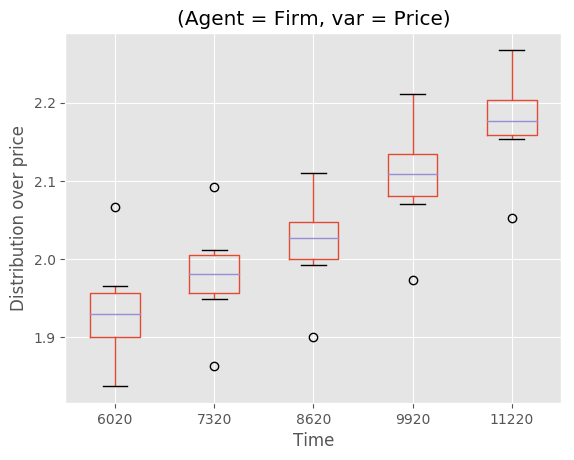
\includegraphics[scale=.7]{./plots_tut_2/one_set_one_run_bp_price_price.png}
\caption{\footnotesize  Example 3: boxplots of the population distribution across 80 agent instances, the number of boxplots can be specified (here: 5).}
\end{figure}

\clearpage
\subsubsection{Example 4}
For agent Firm, one set, 20 runs, 80 agent instances, scatter plot of two variables.

\begin{lstlisting}
config.yaml::

    plot4:
        scatterplot:
            agent: Firm
            analysis: multiple_batch
            variables:
                var1: [price]
                var2: [output]
            delay: no    
            set: [13]
            run: [range,[1,20]]
            major: [range,[6020,12500,20]]
            minor: [range,[1,80]] 
            summary: mean

plot.yaml::

    plot4:
        number_plots: one
        plot_name: one_set_multiple_runs_sp_price_output.png
        plot_legend: yes
        legend_location: best
        legend_label: price vs. output
        linestyle: solid
        marker: +
\end{lstlisting}

\begin{figure}[b!]\centering\leavevmode
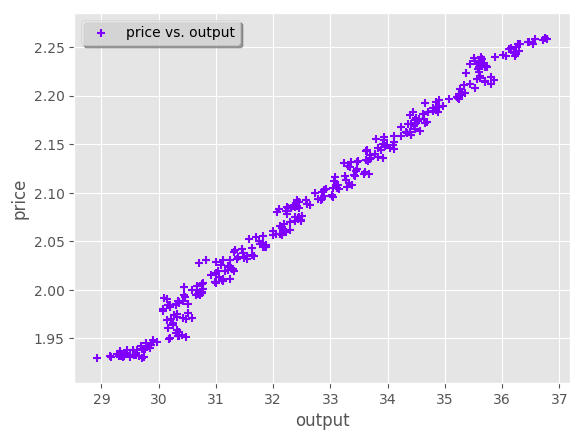
\includegraphics[scale=.7]{./plots_tut_2/one_set_multiple_runs_sp_price_output_0.png}
\caption{\footnotesize  Example 4: Scatter plot of 2 variables, for a data set consisting of 20 runs, 80 agent instances. We first took the mean across the agents, then plot the ensemble data across all runs, and all iterations (the plot shows $20\times 325$ points).}
\end{figure}

\clearpage
\subsubsection{Example 5}
 For agent Firm, one set, 20 runs each, 80 agent instances, delay plot for one variable.

\begin{lstlisting}
config.yaml::

    plot5:
        scatterplot:
            agent: Firm
            analysis: multiple_batch
            variables:
                var1: [price]
            delay: yes
            set: [13]
            run: [range,[1,20]]
            major: [range,[6020,12500,20]]
            minor: [range,[1,80]] 
            summary: mean

plot.yaml::

    plot5:
        number_plots: one
        plot_name: one_set_multiple_runs_sp_price_delay.png
        plot_legend: yes
        legend_location: best
        legend_label: price vs. price_delay
        linestyle: solid
        marker: +
\end{lstlisting}

\begin{figure}[b!]\centering\leavevmode
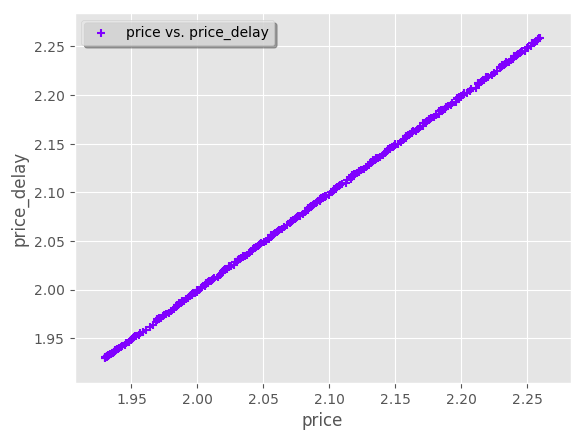
\includegraphics[scale=.7]{./plots_tut_2/one_set_multiple_runs_sp_price_delay_0.png}
\caption{\footnotesize  Example 5: Delay plot $(x_t, x_{t+1})$.}
\end{figure}

\clearpage
\subsubsection{Example 6}
For agent Firm, one set, one run, 80 agent instances, histogram of one variable.

\begin{lstlisting}
config.yaml::

    plot6:
        histogram:
            agent: Firm
            analysis: multiple_run
            variables:
                var1: [price]
            set: [10]
            run: [1]
            major: [range,[6020,12500,20]]
            minor: [range,[1,80]] 
            summary: mean

plot.yaml::

    plot6:
        number_plots: one
        plot_name: one_set_one_run_hg_price.png
        plot_title: (Agent = Firm, var = Price)
        number_bins: 50
        histtype: bar
        plot_legend: yes
        fill: yes
        stacked: False
        legend_location: best
        xaxis_label: xlabel
        yaxis_label: ylabel
\end{lstlisting}

\begin{figure}[b!]\centering\leavevmode
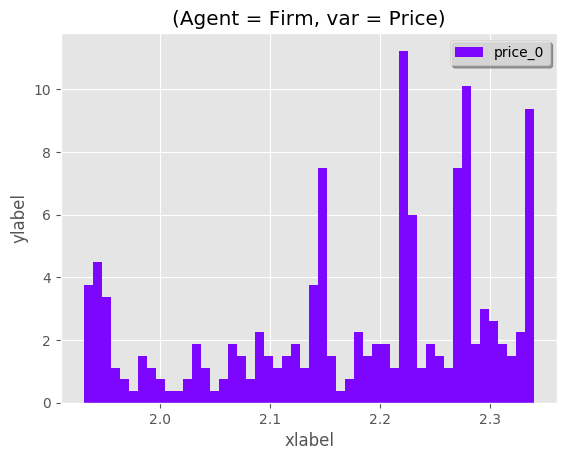
\includegraphics[scale=.7]{./plots_tut_2/one_set_one_run_hg_price_price.png}
\caption{\footnotesize  Example 6: Histogram of a single variable across the agent population.}
\end{figure}

\clearpage
\subsubsection{Example 7}
 For agent Firm, one set, 20 runs, 80 agent instances, histogram of the ensemble distribution over all sets.

\begin{lstlisting}
config.yaml::

    plot7:
        histogram:
            agent: Firm
            analysis: multiple_set
            variables:
                var1: [price]
            set: [10]
            run: [range,[1,20]]
            major: [range,[6020,12500,20]]
            minor: [range,[1,80]] 
            summary: mean

plot.yaml::

    plot7:
        number_plots: one
        plot_name: one_set_multiple_runs_hg_price.png
        plot_title: (Agent = Firm, var = Price)
        number_bins: 50
        histtype: step
        plot_legend: yes
        fill: no
        stacked: False
        legend_location: best
        xaxis_label: xlabel
        yaxis_label: ylabel
\end{lstlisting}

\begin{figure}[b!]\centering\leavevmode
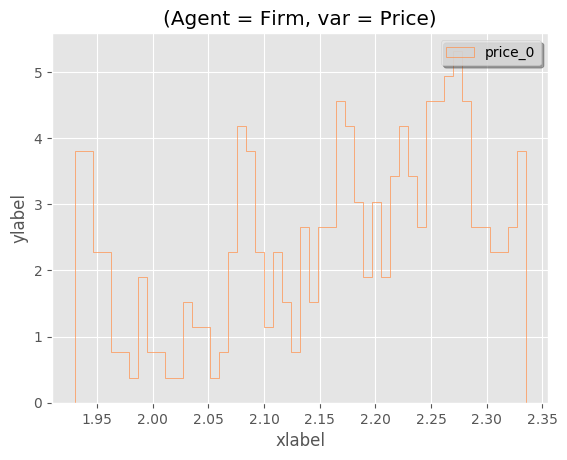
\includegraphics[scale=.6]{./plots_tut_2/one_set_multiple_runs_hg_price_price.png}
\caption{\footnotesize  Example 7: Histogram of a single variable across 20 runs, and across the agent population. Shown is the ensemble distribution across all runs, by concatenating and flattening the data across all dimensions.}
\end{figure}


\clearpage
\subsubsection{Example 8}
For agent Firm, four sets, 20 runs each, 80 agent instances, the variable price is plotted in a single plot.

\begin{lstlisting}
config.yaml::

    plot8:
        timeseries:
            agent: Firm
            analysis: multiple_batch
            variables:
                var1: [output]
            set: [10,13,16,17]
            run: [range,[1,20]]
            major: [range,[6020,12500,20]]
            minor: [range,[1,80]] 
            summary: mean

plot.yaml::

    plot8:
        number_plots: one
        plot_name: timeseries_agentanalysis.png
        plot_legend: yes
        legend_location: best
        x-axis label: Time
        y-axis label: output
        linestyle: dashed
        marker: None
\end{lstlisting}

\begin{figure}[b!]\centering\leavevmode
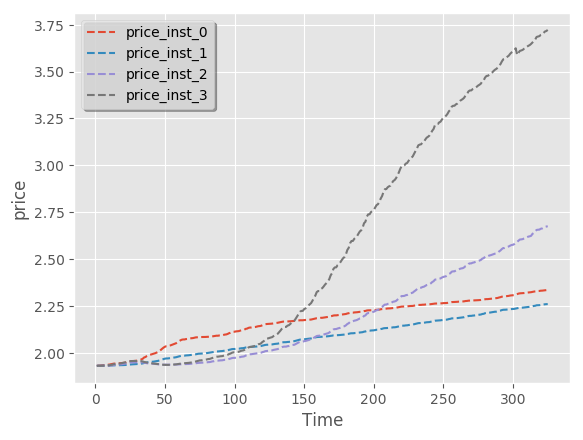
\includegraphics[scale=.6]{./plots_tut_2/P4_ts_price.png}
\caption{\footnotesize  Example 8: Time series plot of multiple sets (4), multiple runs (20), and multiple agent instances (80). Each line represents one set, and displays the mean across runs, and across agents.}
\end{figure}



\clearpage
\subsubsection{Example 9}
For agent Firm, 4 sets, 20 runs each, 80 agent instances, 20-80 quantiles of the population distribution of the variable price are plotted in a single plot.

\begin{lstlisting}
config.yaml::

    plot7:
        timeseries:
            agent: Firm
            analysis: multiple_batch
            variables:
                var1: [price]
            set: [10,13,16,17]
            run: [range,[1,20]]
            major: [range,[6020,12500,20]]
            minor: [range,[1,80]] 
            summary: custom_quantile
            quantile_values:          
                lower_quantile : 0.20
                upper_quantile : 0.80


plot.yaml::

    plot7:
        number_plots: one
        plot_name: ts_multibatch_analysis.png
        plot_legend: yes
        legend_location: best
        x-axis label: Time
        y-axis label: price
        linestyle: solid
        marker: None
        fill_between_quartiles: yes
\end{lstlisting}

\begin{figure}[b!]\centering\leavevmode
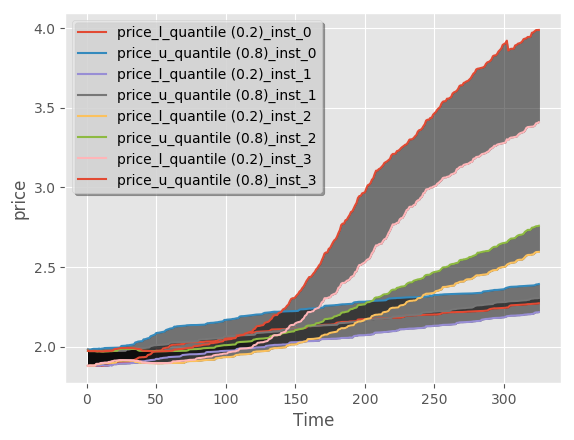
\includegraphics[scale=.6]{./plots_tut_2/P7_ts_price.png}
\caption{\footnotesize  Example 9: Quantile ranges of the variable 'price' for multiple sets (4), multiple runs (20), and multiple agent instances (80). For each set the quantile range (20-80) is displayed.}
\end{figure}


\section{FLAViz FAQ}

\begin{itemize}
\item[Q:] Why is FLAViz based on Python pandas and matplotlib?

A: Python pandas is open source, has an active user community, and has many developers. It is the current library of choice for time series data analysis.
It provides many build-in statistical functionalities.
There are two main functionalities of pandas that are especially important for us:

\begin{itemize}
\item hierarchical indexing: this allows us to use a high dimensional data frame (the ndarray format).
\item bygroup: this allows us to rotate the hierarchical index.
\end{itemize}

\item[Q:] Why the conversion from XML files to HDF5 format?

A: The XML files that FLAME outputs is a fully tagged data format, so it is very verbose. For large scale simulations this is prohibitive, due to the sheer size of the data volumes this generates.
To reduce this storage footprint, but still keep all data together in a structured format, the HDF5 standard was chosen for its hierarchical structure.
The data for each agent type is stored in a single HDF5 file, which can be of any size (we have so far dealt with single files of up to 20 GB without any problems).
Inside of the HDF5 file there is a POSIX-style folder hierarchy, with data groups and data sets. A particular requirement for HDF5 is that the 'data set' has a homogeneous data structure.
For this data structure we have selected the 3D DataFrame from Python pandas (but we should note that the current development of Python pandas goes soo quick that currently this is shifting to the ndarray, which will replace the 3D Data Panel in a more generic data format).

\item[Q:] How do you do the data transformations, data selection and data filtering?

We use the bygroup function of pandas to sort the hierarchical index, and to rotate the data frame.

\item[Q:] Can I use FLAViz with other agent-based simulation platforms than FLAME?

Yes, you can! The only requirement is that the final data output is either in XML or in HDF5 format (see the file format specifications).
\end{itemize}

\end{document}
